% !TeX root = thesis.tex
%%%%%%%%%%%%%%%%%%%%%%%%%%%%%%%%%%%%%%%%%%%%%%%%%%%%%%%%%%%%%%%%%%%%%%%%
%                                                                      %
% LaTeX, FIIW thesis template                                          %
% 14/03/2023 v1.3                                                      %
%                                                                      %
%%%%%%%%%%%%%%%%%%%%%%%%%%%%%%%%%%%%%%%%%%%%%%%%%%%%%%%%%%%%%%%%%%%%%%%%
\documentclass[11pt,a4paper]{report}
% Indien je je thesis recto-verso wil afdrukken gebruik je onderstaande opties i.p.v. bovenstaande
%\documentclass[11pt,a4paper,twoside,openright]{report}
\usepackage[a4paper,left=3.5cm, right=2.5cm, top=3.5cm, bottom=3.5cm]{geometry}
\usepackage{graphicx}
\graphicspath{{./figs/}}                % set graphics path to figs folder, ie now all file imports can be referenced relative to figs
\usepackage[latin1]{inputenc}           % om niet ascii karakters rechtstreeks te kunnen inputten
%\usepackage[utf8]{inputenc}            % commentarieer deze regel uit als je utf8 encoded files gebruikt in plaats van latin1
\usepackage[backend=biber, style=ieee, citestyle=numeric-comp, maxnames=99]{biblatex}
\addbibresource{bib.bib}
\AtBeginBibliography{\footnotesize}
\usepackage{cmbright} % new improved font
\usepackage{listings}             		% voor het weergeven van broncode
\usepackage[outputdir=cache]{minted}                     % for beautiful listings
\usemintedstyle{borland}
\usepackage{verbatim}					% weergeven van code, commando's, ...
\usepackage{hyperref}					% maak PDF van de thesis navigeerbaar
\usepackage{url}						% URL's invoegen in tekst met behulp van \url{http://}
\usepackage[small,bf,hang]{caption}     % om de captions wat te verbeteren
\usepackage[final]{pdfpages}            % gebruikt voor het invoegen van het artikel in pdf-formaat
%\usepackage{pslatex}					% andere lettertype's dan de standaard types

%\usepackage{sectsty}					% aanpassen van de fonts van sections en chapters
%\allsectionsfont{\sffamily}
%\chapterfont{\raggedleft\sffamily}

\usepackage{float}                      % De optie H voor de plaatsing van figuren op de plaats waar je ze invoegt. bvb. \begin{figure}[H]
%\usepackage{longtable}					% tabellen die over meerdere pagina's gespreid worden
%\usepackage[times]{quotchap}           % indien je fancy hoofdstuktitels wil
%\usepackage[none]{hyphenat}
%\usepackage{latexsym}
\usepackage{amsmath}
\usepackage{amssymb}
\usepackage{siunitx}
\sisetup{detect-all}
\usepackage[acronym,xindy]{glossaries}
\makenoidxglossaries
\usepackage[version=4]{mhchem} % chemical formulas
\usepackage{tabularx}
\usepackage{booktabs} % nice tables
\usepackage{array} % fixed-width columns in tables

%%%% Tikz %%%%
\usepackage{pgfplots}
\DeclareUnicodeCharacter{2212}{−}
\usepgfplotslibrary{groupplots,dateplot}
\usetikzlibrary{patterns,shapes.arrows}
\pgfplotsset{compat=newest}
%%%%%%%%%%%% MAKE FIGURES MORE UNIFORM %%%%%%%%%%%%
\definecolor{darkgray176}{RGB}{176,176,176}
\definecolor{color0}{RGB}{255,127,14}
\definecolor{color1}{RGB}{44,160,44}
\pgfplotsset{
    every axis/.append  style={
        title style={draw=none},
        label style={font=\small},
        legend style={
            fill opacity=0.8,
            nodes={scale=0.8, transform shape}, {draw=none}
        },
        tick align=outside,
        tick pos=left,
        x grid style={darkgray176},
        xtick style={color=black},
        y grid style={darkgray176},
        ytick style={color=black},
        grid=both,
    },
    every axis plot/.append style={
        line width=1.0pt,
        mark size=1,
    },
}



%%%%%%%%%%%% choose your campus and language %%%%%%%%%%%%
\usepackage{fiiw} 



%door onderstaande regels in commentaar te zetten, of op false, kan je pagina's weglaten
%bijvoorbeeld het weglaten van een voorwoord, lijst met symbolen, ...
%%%%%%%%%%%%%%%%%%%%%%%%%%%%%%%%%%%%%%%%%%%%%%%%%%%%%%%%%%%%%%%%%%%%%%%%%%%%%%%%%%%%%%%%
%voorwoord toevoegen?
\acknowledgementspagetrue
\acknowledgements{voorwoord}			%.tex file met daarin het voorwoord
%abstract toevoegen?
\abstractpagetrue
\abstracts{abstract}					%.tex file met daarin het abstract
%lijst van figuren toevoegen?
%\listoffigurespagetrue
%lijst van tabellen toevoegen?
%\listoftablespagetrue
%lijst van symbolen toevoegen?
%\listofsymbolspagetrue
%\listofsymbols{symbolen}				%.tex file met daarin de lijst van symbolen


%informatie over het eindwerk, de promotor, ...
%%%%%%%%%%%%%%%%%%%%%%%%%%%%%%%%%%%%%%%%%%%%%%%
\opleiding{naam opleiding}
\afdeling{afstudeerrichting}
\campus{ghenteng}
\title{Titel Masterproef}
\subtitle{Ondertitel (facultatief)}
\forenameA{Sien}
\surnameA{Peerlinck}
\forenameB{} %keep empty if no 2nd author
\surnameB{} %keep empty if no 2nd author
\academicyear{2023 - 2024}


\promotorA[Promotor(en)]{Dr. Geoffrey Ottoy} %for English use Supervisor(s)
\promotorB[Co-promotor(en)]{Sophie Berkenbosch}

% generated by Gilles Callebaut with the script: https://github.com/DRAMCO/writing-scientific-papers-in-latex-tips-and-tricks/blob/main/glossaries/merge_abbr.py

%%%%%%%%%%%% 2 %%%%%%%%%%%%
\newacronym{2d}{2D}{two-dimensional}
%%%%%%%%%%%% 3 %%%%%%%%%%%%
\newacronym{3d}{3D}{three-dimensional}
\newacronym{3gpp}{3GPP}{3rd generation partnership project}
%%%%%%%%%%%% 5 %%%%%%%%%%%%
\newacronym{5g}{5G}{fifth-generation}
%%%%%%%%%%%% 6 %%%%%%%%%%%%
\newacronym{6g}{6G}{sixth-generation}
%%%%%%%%%%%% A %%%%%%%%%%%%
\newacronym{abp}{ABP}{authentication by personalisation}
\newacronym{aclr}{ACLR}{adjacent channel leakage ratio}
\newacronym{adc}{ADC}{Analog-to-digital converter}
\newacronym{adr}{ADR}{adaptive data rate}
\newacronym{aec}{AEC}{Adaptive Entropy Coder}
\newacronym{ag}{AG}{array gain}
\newacronym{ai}{AI}{artificial intelligence}
\newacronym{amam}{AM/AM}{amplitude modulation to amplitude modulation}
\newacronym{amp}{AMP}{approximate message passing}
\newacronym{ampm}{AM/PM}{amplitude modulation to phase modulation}
\newacronym{aoa}{AOA}{angle-of-arrival}
\newacronym{aod}{AOD}{angle-of-departure}
\newacronym{ap}{AP}{access point}
\newacronym{apu}{APU}{access point unit}
\newacronym{ar}{AR}{augmented reality}
\newacronym{arp}{ARP}{Antenna Reference Point}
\newacronym{asic}{ASIC}{application specific integrated circuit}
\newacronym{ask}{ASK}{amplitude-shift keying}
\newacronym{auv}{AUV}{autonomous underwater vehicle}
\newacronym{awgn}{AWGN}{additive white Gaussian noise}
%%%%%%%%%%%% B %%%%%%%%%%%%
\newacronym{baw}{BAW}{bulk acoustic wave}
\newacronym{bb}{BB}{base-band}
\newacronym{bf}{BF}{beamforming}
\newacronym{bldc}{BLDC}{brushless DC}
\newacronym{bom}{BOM}{bill of materials}
\newacronym{bs}{BS}{base station}
\newacronym{bw}{BW}{bandwidth}
%%%%%%%%%%%% C %%%%%%%%%%%%
\newacronym{cad}{CAD}{channel activity detection}
\newacronym{cars}{CARS}{calibration reference signal}
\newacronym{cbm}{CBM}{condition based maintenance}
\newacronym{cc}{CC}{constant current}
\newacronym{ccdf}{CCDF}{complementary cumulative distribution function}
\newacronym{ccnn}{CCNN}{circular convolutional neural network}
\newacronym{ccs}{CCS}{correlative channel sounder}
\newacronym{ccsds}{CCSDS}{Consultative Committee for Space Data Systems}
\newacronym{cdf}{CDF}{cumulative distribution function}
\newacronym{cdrx}{CDRX}{connected mode DRX}
\newacronym{ce}{CE}{coverage enhancement}
\newacronym{ced}{CED}{cumulative energy density}
\newacronym{cf}{CF}{cell-free}
\newacronym{cfo}{CFO}{carrier frequency offset}
\newacronym{cir}{CIR}{channel impulse response}
\newacronym{cost}{COST}{commercial off-the-shelf}
\newacronym{cots}{COTS}{commercial off-the-shelf}
\newacronym{cp}{CP}{cyclic prefix}
\newacronym{cpt}{CPT}{capacitive power transfer}
\newacronym{cpu}{CPU}{central-processing unit}
\newacronym{cqi}{CQI}{channel quality indicator}
\newacronym{cr}{CR}{coding rate}
\newacronym{crlb}{CRLB}{Cram\'er-Rao lower bound}
\newacronym{crs}{CRS}{cell reference signal}
\newacronym{cs}{CS}{compressed sensing}
\newacronym{csi}{CSI}{channel state information}
\newacronym{csp}{CSP}{contact service point}
\newacronym{css}{CSS}{chirp spread spectrum}
\newacronym{cv}{CV}{constant voltage}
%%%%%%%%%%%% D %%%%%%%%%%%%
\newacronym{dac}{DAC}{digital-to-analog converter}
\newacronym{daq}{DAQ}{data acquisition system}
\newacronym{dc}{DC}{direct current}
\newacronym{dcc}{DCC}{dynamic cooperation clustering}
\newacronym{de}{DE}{drain efficiency}
\newacronym{dl}{DL}{downlink}
\newacronym{dlc}{DLC}{Distributed Laser Charging}
\newacronym{dma}{DMA}{Direct Memory Access}
\newacronym{dmimo}{D-MIMO}{distributed MIMO}
\newacronym{dpd}{DPD}{digital pre-distortion}
\newacronym{dpdk}{DPDK}{Data Plane Development Kit}
\newacronym{drx}{DRX}{Discontinuous Reception Mode}
\newacronym{duc}{DUC}{digital up-converter}
\newacronym{dwt}{DWT}{discrete wavelet transform}
%%%%%%%%%%%% E %%%%%%%%%%%%
\newacronym{e2e}{E2E}{end-to-end}
\newacronym{easa}{EASA}{European Union Aviation Safety Agency}
\newacronym{ecdf}{eCDF}{empirical cumulative distribution function}
\newacronym{ecsp}{ECSP}{edge computing service point}
\newacronym{edlc}{EDLC}{electrostatic double-layer capacitors}
\newacronym{edrx}{eDRX}{Extended Discontinuous Reception Mode}
\newacronym{ee}{EE}{energy efficiency}
\newacronym{egprs}{EGPRS}{Enhanced Data Rates for GSM Evolution}
\newacronym{eirp}{EIRP}{effective isotropic radiated power}
\newacronym{em}{EM}{electromagnetic}
\newacronym{embb}{eMBB}{enhanced Mobile Broadband}
\newacronym{en}{EN}{energy neutral}
\newacronym{eol}{EoL}{end of life}
\newacronym{epu}{EPU}{edge processing unit}
\newacronym{erp}{ERP}{effective radiated power}
\newacronym[plural=ESCs,firstplural=electronic speed controllers (ESCs)]{esc}{ESC}{electronic speed control}
\newacronym{etsi}{ETSI}{European Telecommunications Standards Institute}
\newacronym{evm}{EVM}{Error Vector Magnitude}
%%%%%%%%%%%% F %%%%%%%%%%%%
\newacronym{fa}{FA}{federation anchor}
\newacronym{fapec}{FAPEC}{Fully Adaptive Prediction Error Coding}
\newacronym{felics}{FELICS}{Fast and Efficient Lossless Image Compression}
\newacronym{fembb}{feMBB}{further enhanced mobile broadband}
\newacronym{fft}{FFT}{fast Fourier transform}
\newacronym{fh}{FH}{fronthaul}
\newacronym{fim}{FIM}{Fisher information matrix}
\newacronym{fom}{FoM}{figure of merit}
\newacronym{fpga}{FPGA}{field-programmable gate array}
%%%%%%%%%%%% G %%%%%%%%%%%%
\newacronym{gb}{GB}{grant-based}
\newacronym{gf}{GF}{grant-free}
\newacronym{gnb}{gNB}{Next Generation Node B}
\newacronym{gnn}{GNN}{graph neural network}
\newacronym{gnss}{GNSS}{global navigation satellite system}
\newacronym{gpclk}{GPCLK}{general purpose clock}
\newacronym{gprs}{GPRS}{General Packet Radio Services}
\newacronym{gps}{GPS}{Global Positioning System}
\newacronym{gpu}{GPU}{graphical processing unit}
\newacronym{gsm}{GSM}{Global System for Mobile Communications}
\newacronym{gwp}{GWP}{Global Warming Potential}
%%%%%%%%%%%% H %%%%%%%%%%%%
\newacronym{harq}{HARQ}{hybrid automatic repeat request}
\newacronym{hat}{HAT}{hardware attached on top}
\newacronym{hcs}{HCS}{human-centric services}
\newacronym{hpbm}{HPBM}{half power beam width}
%%%%%%%%%%%% H %%%%%%%%%%%%
\newacronym{HyMPRo}{HyMPRo}{Hybrid Multi-Path Routing algorithm}
%%%%%%%%%%%% I %%%%%%%%%%%%
\newacronym{ib}{IB}{in-band}
\newacronym{ibo}{IBO}{input back-off}
\newacronym{ic}{IC}{integrated circuit}
\newacronym{id}{ID}{information decoding}
\newacronym{if}{IF}{intermediate-frequency}
\newacronym{iid}{i.i.d.}{independently and identically distributed}
\newacronym{im}{IM}{intermodulation}
\newacronym{imu}{IMU}{inertial measurement unit}
\newacronym{io}{IO}{input/output}
\newacronym{iot}{IoT}{Internet of Things}
\newacronym{ipt}{IPT}{inductive power transfer}
\newacronym{ipy}{IPY}{Interventions per Year}
\newacronym{iq}{IQ}{in-phase and quadrature}
\newacronym{ir}{IR}{infrared}
\newacronym{ism}{ISM}{industrial, scientific and medical}
\newacronym{isp}{ISP}{internet service provider}
%%%%%%%%%%%% K %%%%%%%%%%%%
\newacronym{kpi}{KPI}{key performance indicator}
\newacronym{kvi}{KVI}{key value indicator}
%%%%%%%%%%%% L %%%%%%%%%%%%
\newacronym{lca}{LCA}{life cycle assessment}
\newacronym{lco}{LCO}{lithium cobalt oxide}
\newacronym{ldo}{LDO}{Low-dropout voltage regulator}
\newacronym{ldpc}{LDPC}{low-density parity-check}
\newacronym{lfp}{LFP}{lithium iron phosphate}
\newacronym{lic}{LIC}{lithium-ion capacitor}
\newacronym{lidar}{LiDAR}{light detection and ranging}
\newacronym{liion}{Li-ion}{lithium-ion}
\newacronym{lipo}{LiPo}{lithium polymer}
\newacronym{lis}{LIS}{large intelligent surface}
\newacronym{llh}{LLH}{log-likelihood}
\newacronym{lmmse}{LMMSE}{least minimum mean square error}
\newacronym{lmo}{LMO}{lithium ion manganese oxide}
\newacronym{lo}{LO}{local oscillator}
\newacronym{lora}{LoRa}{long range}
\newacronym{lorawan}{LoRaWAN}{long-range wide-area network}
\newacronym{los}{LoS}{line-of-sight}
\newacronym{lp}{LP}{linear programming}
\newacronym{lpt}{LPT}{laser power transfer}
\newacronym{lpwa}{LPWA}{Low Power Wide Area}
\newacronym{lpwan}{LPWAN}{low-power wide-area network}
\newacronym{lqi}{LQI}{link quality indicator}
\newacronym{lrelu}{LReLU}{leaky rectified linear unit}
\newacronym{lrt}{LRT}{likelihood-ratio test}
\newacronym{ls}{LS}{least squares}
\newacronym{lsa}{LSA}{large synthetic array}
\newacronym{lsfc}{LSFC}{large-scale fading component}
\newacronym{ltc}{LTC}{lithium thionyl chloride}
\newacronym{lte}{LTE}{Long Term Evolution}
\newacronym{lto}{LTO}{lithium titanate}
%%%%%%%%%%%% M %%%%%%%%%%%%
\newacronym{m2m}{M2M}{machine to machine}
\newacronym{mac}{MAC}{Medium Access Control}
\newacronym{mate}{MATE}{millimeter-wave MIMO testbed}
\newacronym{mcl}{MCL}{Maximum Coupling Loss}
\newacronym{mcs}{MCS}{modulation and coding scheme}
\newacronym{mcu}{MCU}{Microcontroller Unit}
\newacronym{mec}{MEC}{multi-access edge computing}
\newacronym{mems}{MEMS}{micro-electromechanical systems}
\newacronym{mf}{MF}{matched filter}
\newacronym{mimo}{MIMO}{multiple-input multiple-output}
\newacronym{miso}{MISO}{multiple-input single-output}
\newacronym{ml}{ML}{machine learning}
\newacronym{mlp}{MLP}{multilayer perceptron}
\newacronym{mmimo}{mMIMO}{massive MIMO}
\newacronym{mmse}{MMSE}{minimum mean square error}
\newacronym{mmtc}{mMTC}{massive machine-typed communication}
\newacronym{mmwave}{mmWave}{millimeter wave}
\newacronym{mpc}{MPC}{multipath component}
\newacronym{mppt}{MPPT}{maximum power point tracking}
\newacronym{mr}{MR}{maximum ratio}
\newacronym{mrc}{MRC}{maximum ratio combining}
\newacronym{mrc_em}{MRC}{maximum ratio combining}
\newacronym{mrc_EM}{MRC}{Magnetic Resonance Coupling}
\newacronym{mrt}{MRT}{maximum ratio transmission}
\newacronym{mse}{MSE}{mean square error}
\newacronym{mtc}{MTC}{Machine-Type Communication}
\newacronym{multi-rat}{Multi-RAT}{multiple radio access technology}
%%%%%%%%%%%% N %%%%%%%%%%%%
\newacronym{nb}{NB}{narrowband}
\newacronym{nbiot}{NB-IoT}{narrowband IoT}
\newacronym{nca}{NCA}{nickel cobalt aluminum}
\newacronym{nicd}{NiCd}{nikkel cadmium}
\newacronym{nimh}{NiMH}{nikkel metal hydride}
\newacronym{nlos}{NLoS}{non-line-of-sight}
\newacronym{nmc}{NMC}{nickel manganese cobalt}
\newacronym{nn}{NN}{neural network}
\newacronym{nnls}{NNLS}{non-negative least squares}
\newacronym{noma}{NOMA}{non-orthogonal multiple access}
\newacronym{nr}{NR}{New Radio}
\newacronym{ntp}{NTP}{network time protocol}
%%%%%%%%%%%% O %%%%%%%%%%%%
\newacronym{oai}{OAI}{OpenAirInterface} % no spelling mistake, it is spelled all glued to eachother...
\newacronym{ofdm}{OFDM}{orthogonal frequency-division multiplexing}
\newacronym{ofdmim}{OFDM-IM}{OFDM with index modulation}
\newacronym{oob}{OOB}{out-of-band}
\newacronym{oran}{O-RAN}{open radio-access network}
\newacronym{os}{OS}{operating system}
\newacronym{ota}{OTA}{over-the-air}
\newacronym{otaa}{OTAA}{over-the-air authentication}
%%%%%%%%%%%% P %%%%%%%%%%%%
\newacronym{p2p}{P2P}{point-to-point}
\newacronym{pa}{PA}{power amplifier}
\newacronym{pae}{PAE}{power-added efficiency}
\newacronym{papr}{PAPR}{peak-to-average power ratio}
\newacronym{pc}{PC}{pilot count}
\newacronym{pcb}{PCB}{printed circuit board}
\newacronym{pcg}{PCG}{power consumption gain}
\newacronym{pd}{PD}{powered device}
\newacronym{pdcch}{PDCCH}{physical downlink control channel}
\newacronym{pdp}{PDP}{power delay profile}
\newacronym{pdsch}{PDSCH}{physical downlink shared channel}
\newacronym{pec}{PEC}{prediction error coding}
\newacronym{per}{PER}{packet error rate}
\newacronym{pg}{PG}{path gain}
\newacronym{pgd}{PGD}{proximal gradient descent}
\newacronym{pl}{PL}{path loss}
\newacronym{pll}{PLL}{phase-locked loop}
\newacronym{poe}{PoE}{power-over-Ethernet}
\newacronym{pps}{1PPS}{pulse per second}
\newacronym{prbs}{PRBs}{Physical Resource Blocks}
\newacronym{ps}{PS}{Processing System}
\newacronym{psd}{PSD}{power spectral density}
\newacronym{pse}{PSE}{power sourcing equipment}
\newacronym{psm}{PSM}{power saving mode}
\newacronym{pss}{PSS}{primary synchronisation signal}
\newacronym{ptp}{PTP}{precision-time protocol}
\newacronym{ptrs}{PTRS}{Phase-Tracking Reference Signals}
\newacronym{ptw}{PTW}{paging time window}
\newacronym{pwm}{PWM}{pulse width modulation}
%%%%%%%%%%%% Q %%%%%%%%%%%%
\newacronym{qam}{QAM}{quadrature amplitude modulation}
\newacronym{qos}{QoS}{quality-of-service}
\newacronym{quadriga}{QuaDRiGa}{QUAsi Deterministic RadIo channel GenerAtor}
%%%%%%%%%%%% R %%%%%%%%%%%%
\newacronym{ra}{RA}{Random Access}
\newacronym{ran}{RAN}{radio access network}
\newacronym{rar}{RAR}{Random Access Response}
\newacronym{rat}{RAT}{radio access technology}
\newacronym{rbs}{RBS}{radio base station}
\newacronym{re}{RE}{radio element}
\newacronym[]{relu}{ReLU}{rectified linear unit}
\newacronym{rf}{RF}{radio frequency}
\newacronym{rfeh}{RFEH}{radio frequency energy harvesting}
\newacronym{rfic}{RFIC}{radio-frequency integrated circuit}
\newacronym{rfid}{RFID}{radio frequency identification}
\newacronym{rfpt}{RFPT}{radio frequency power transfer}
\newacronym{rfsoc}{RFSoC}{Radio Frequency System-on-Chip}
\newacronym{ris}{RIS}{reflective intelligent surface}%reconfigurable?
\newacronym{rllmtc}{RLLMTC}{reliable low latency machine type communication}
\newacronym{rms}{RMS}{root-mean-square}
\newacronym{rmse}{RMSE}{root-mean-square error}
\newacronym{rof}{RoF}{radio-over-fiber}
\newacronym{ros}{ROS}{robot operating system}
\newacronym{rpi}{RPi}{Raspberry Pi}
\newacronym{rrc}{RRC}{Radio Resource Connection}
\newacronym{rreq}{RREQ}{route request packet}
\newacronym{rsrp}{RSRP}{Reference Signals Received Power}
\newacronym{rss}{RSS}{received signal strength}
\newacronym{rssi}{RSSI}{received signal strength indicator}
\newacronym{rtc}{RTC}{real time clock}
\newacronym{rtk}{RTK}{real time kinematics}
\newacronym{rts}{RTS}{ray tracing simulator}
\newacronym{rw}{RW}{RadioWeaves}
\newacronym{rx}{RX}{receiver}
\newacronym{rzf}{RZF}{regularized zero forcing}
%%%%%%%%%%%% S %%%%%%%%%%%%
\newacronym{sa}{SA}{synchronization anchor}
\newacronym{scfdma}{SCFDMA}{single-carrier frequency division multiple access}
\newacronym{sdg}{SDG}{Sustainable Development Goal}
\newacronym{sdm}{SDM}{sigma-delta modulator}
\newacronym{sdn}{SDN}{software-defined network}
\newacronym{sdof}{SDoF}{sigma-delta over fiber}
\newacronym{sdr}{SDR}{software-defined radio}
\newacronym{sf}{SF}{spreading factor}
\newacronym{sfn}{SFN}{single frequency network}
\newacronym{sfp}{SFP}{small form-factor pluggable}
\newacronym{sinr}{SINR}{signal-to-interference-plus-noise ratio}
\newacronym{siso}{SISO}{single-input single-output}
\newacronym{slam}{SLAM}{simultaneous localization and mapping}
\newacronym{slc}{SLC}{spatial leakage suppression}
\newacronym{smc}{SMC}{specular multipath component}
\newacronym{smps}{SMPS}{switched mode power supply}
\newacronym{sndr}{SNDR}{signal-to-noise-and-distortion ratio}
\newacronym{snidr}{SNIDR}{signal-to-noise-and-interference-and-distortion ratio}
\newacronym{snr}{SNR}{signal-to-noise ratio}
\newacronym{soc}{SoC}{state of charge}
\newacronym{ssb}{SSB}{synchronisation signal block}
\newacronym{ssd}{SSD}{solid state drive}
\newacronym{steam}{STEAM}{science, technology, engineering, the arts, and mathematics}
\newacronym{svd}{SVD}{singular value decomposition}
%%%%%%%%%%%% T %%%%%%%%%%%%
\newacronym{tau}{TAU}{tracking area update}
\newacronym{tcer}{TCER}{transported to consumed energy ratio}
\newacronym{tdd}{TDD}{time division duplexing}
\newacronym{tdoa}{TDOA}{time-difference-of-arrival}
\newacronym{toa}{TOA}{time-of-arrival}
\newacronym{tof}{ToF}{time-of-flight}
\newacronym{tosm}{TOSM}{through-open-short-match}
\newacronym{trl}{TRL}{technology readyness level}
\newacronym{trp}{TRP}{Transmission Reception Point}
\newacronym{tsn}{TSN}{time-sensitive networking}
\newacronym{ttm}{TTM}{time to market}
\newacronym{ttn}{TTN}{The Things Network}
\newacronym{tx}{TX}{transmitter}
%%%%%%%%%%%% U %%%%%%%%%%%%
\newacronym{uav}{UAV}{unmanned aerial vehicle}
\newacronym{udp}{UDP}{User Datagram Protocol}
\newacronym{unitdp}{UDP}{Unit-Delay Predictor}
\newacronym{ue}{UE}{user equipment}
\newacronym{ugv}{UGV}{unmanned ground vehicle}
\newacronym{uhd}{UHD}{USRP hardware driver}
\newacronym{uhf}{UHF}{ultra-high frequency}
\newacronym{ul}{UL}{uplink}
\newacronym{ula}{ULA}{uniform linear array}
\newacronym{ummtc}{umMTC}{ultra massive machine type communication}
\newacronym{upa}{UPA}{uniform planar array}
\newacronym{ura}{URA}{uniform rectangular array}
\newacronym{urllc}{URLLC}{ultra-reliable low-latency communications}
\newacronym{usrp}{USRP}{universal software radio peripheral}
\newacronym{uv}{UV}{unmanned vehicle}
\newacronym{uwb}{UWB}{ultrawideband}
%%%%%%%%%%%% V %%%%%%%%%%%%
\newacronym{vep}{VEP}{virtual edge platform}
\newacronym{vlc}{VLC}{visible light communication}
\newacronym{vlp}{VLP}{visible light positioning}
\newacronym{vna}{VNA}{vector network analyzer}
\newacronym{vr}{VR}{virtual reality}
%%%%%%%%%%%% W %%%%%%%%%%%%
\newacronym{wb}{WB}{wideband}
\newacronym{wpt}{WPT}{wireless power transfer}
\newacronym{wr}{WR}{White Rabbit}
\newacronym{wrsn}{WRSN}{wireless rechargeable sensor network}
\newacronym{wsn}{WSN}{wireless sensor network}
%%%%%%%%%%%% X %%%%%%%%%%%%
\newacronym{xr}{XR}{extended reality}
%%%%%%%%%%%% Z %%%%%%%%%%%%
\newacronym{z3ro}{Z3RO}{zero third-order distortion}
\newacronym{zf}{ZF}{zero-forcing}
\newacronym{zmcscg}{ZMCSCG}{zero mean circularly symmetric complex Gaussian}


\begin{document}
\preface

\printnoidxglossary[type=\acronymtype]%
\clearpage

% !TeX root = thesis.tex
% Dit hoofdstuk bevat typisch drie delen.

% Situering van het eindwerk. Hierbij worden de context en de probleemstelling geschetst op %
% attractieve manier zodat ook interesse kan opgewekt worden bij niet experten.

% Formuleren van doelstellingen. Je formuleert een aantal heel concrete doelstellingen die je wilt realiseren binnen je eindwerk. Dit kan in puntjes. De lezer moet bij het lezen van de tekst kunnen aftoetsen of die doelstellingen zijn gehaald.

% Overzicht van de tekst. Je schetst op welke manier de rest van de tekst is gestructureerd. Dit kan door elk hoofdstuk samen te vatten in een aantal lijnen, en de samenhang tussen de hoofdstukken te duiden.


%Het eerste hoofdstuk van je thesis.
\chapter{Introduction}\label{ch:introduction}

% !TeX root = thesis.tex
% Werking en functionaliteit van het systeem. Allereerst moeten er concrete vereisten opgelegd worden aan het systeem. Deze zullen later dan afgetoetst kunnen worden bij de realisatie van het ontwerp.

% De opgestelde vereisten van het systeem kunnen nadien vertaald worden in specificaties die je gebruikt om keuzes te maken in de ontwerpfase (H4).
%second chapter of your thesis
\chapter{Analyse}\label{ch:analyse}

% !TeX root = thesis.tex

% Vermijd bij dit hoofdstuk zeker kopieerwerk van bestaande documenten. Haal veeleer aan op welke manier de bouwblokken worden ingezet. Waar nodig refereren naar andere documenten of URL’s!

% Technologische bouwblokken. Overzicht van technologieën en methodologieën die relevant zijn voor de rest van je eindwerk. Begin met de helicopterview en zoom daarna in op de componenten die echt relevant zijn voor de rest van het eindwerk.

% Gerelateerd werk. Doe een scan van bestaand werk in je domein. Haal aan waar jouw oplossing verschilt t.o.v. bestaande oplossingen.

% Besluit.

 
\chapter{State of the art}\label{ch:sota}

\section{CCSDS}
The \gls{ccsds} is an international organisation of space agencies that formulate solutions for common problems in the development and operation of space data systems \cite{noauthor_ccsdsorg_nodate-1}. These solutions are called ''Recommended Standards''. % Nog meer uitleg want dees is maar mager 

The standards most related to this assignment are discussed below.

\subsection{CCSDS 121.0-b-3}
The \gls{ccsds} 121.0-b-3 recommended standard from august 2020 \cite{ccsds_secretariat_lossless_2020} is a lossless source coding data compression algorithm. It consists of two stages, the first stage being a preprocessor and the second stage an \gls{aec}.

The preprocessor's role is to convert the data by decorrelating and converting it into nonnegative integers with the preferred probability distribution. For the \gls{aec} a probability distribution approaching Laplacian is optimal. The preprocessor presented in this recommended standard is the \gls{unitdp}. This technique predicts the current sample using the one-sample delayed input data signal, this is illustrated in figure \ref{fig:udp}. 
\begin{figure}[h]
    \centering
    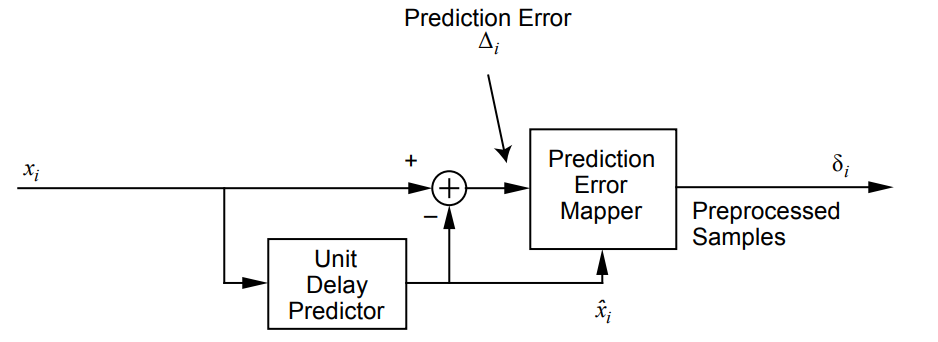
\includegraphics[width=0.7\textwidth]{figs/unit_delay_predictor.png}
    \caption{\acrfull{unitdp} \cite{ccsds_secretariat_lossless_2020}}
    \label{fig:udp}
\end{figure}


\subsection{CCSDS 122.0-b-2}
The \gls{ccsds} 1212.0-b-2 recommended standard from september 2017 \cite{ccsds_secreteriat_image_2017} is an image compression algorithm.

\subsection{Tests}


\section{FAPEC}
\subsection{Algorithm}
\gls{fapec} was developed by Portell, Villafranca and Garc\'{i}a-Berro \cite{portell_fapec_2018} as a way to overcome the problems of the CCSDS 121.0 Lossless Data Compression Recommendation. The idea behind \gls{fapec} was designing an algorithm that is capable of dealing with noise and outliers \cite{villafranca_fapec_2011}. It was made fully adaptive to automatically calibrate the algorithm to the statistics of the data, thus adapting to changes in the data distribution and becoming an completely autonomous coder.

The algorithm itself consists of a pre-processing (or decorrelation) stage followed by a coding stage \cite{portell_fapec_2018}. The pre-processing stage is oiften implemented by a data prediction algorithm or a transform such as the \gls{dwt}. In general this stage generates one output value for each input value. 
The \gls{fapec} core performs a statistical analysis on all individual prediction error blocks, identifying the morst effective coding tables and finally calling the \gls{pec} kernel, which produces a variable-length codefor each of the values to be coded. \gls{pec}

A more in-depth description of the algorithm can be found in \cite{portell_fapec_2018,villafranca_prediction_2013,villafranca_fapec_2011}.


\subsection{Tests}

\section{FELICS}
\subsection{Algorithm}
\gls{felics} is a technique presented by Paul G. Howard and Jeffrey Scott Vitter \cite{howard_fast_1993}.
\begin{figure}[h]
    \centering
    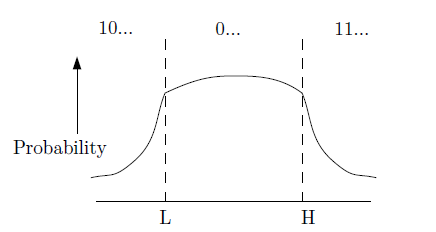
\includegraphics[width=0.5\textwidth]{figs/probability_intensity_P.png}
    \caption{Intensity distribution of new pixel \cite{howard_fast_1993}}
    \label{fig:dist}
\end{figure}
Each pixel is assigned a code depending on where its intensity (grey-scale value) is located relative to the intensities of its closest neighbours. The distribution of an image's intensity distribution is shown in figure \ref{fig:dist}. L denotes the smaller neighbouring intensity value, H denotes the larger neighbouring intensity value. There are three cases:
\begin{enumerate}
    \item The pixel's intensity P lies in the range [L, H]. One bit (0) is used to indicate the in-range position. Since the values of P are almost uniformly distributed, P is assigned an adjusted binary code that is slightly shorter at the centre of the region \cite{salomon_image_2010}.
    \item The pixel's intensity P is lower than L. Now, one bit (1) is used to indicate the out-of-range position, and one bit (0) is used to indicate the below-range position. 
    \item The pixel's intensity P is higher than H. Now, one bit (1) is used to indicate the out-of-range position, and one bit (1) is used to indicate the above-range position.  
\end{enumerate}

The probability of out-of-range values falls off sharply, making it reasonable to use exponential prefix codes like Golomb or Rice codes \cite{howard_fast_1993}.
A formal description of the algorithm can be found in \cite{howard_fast_1993}.

\subsection{Tests}


\section{mijn eigen ding}
\subsection{Algorithm}

\subsection{Tests}

\section{Hardware versus software-implementation}

\section{Conclusion}
% hierin korte samenvatting van de tests en zo vergelijking tussen de verschillende algoritmes maken
% NIETS NIEUWS VERTELLEN
% !TeX root = thesis.tex
% In dit hoofdstuk geef je een overzicht van het ontwerp van je oplossing. De manier waarop dit hoofdstuk wordt gestructureerd is afhankelijk van het systeem onder studie. Begin opnieuw met een helicopterview die een overzicht geeft van het ganse ontwerp, en zoom daarna in op deelaspecten of componenten. Reflecteer daarna over de genomen ontwerpbeslissingen, en mogelijke alternatieven. Bestudeer de toepasbaarheid van de geselecteerde componenten op basis van de vooropgestelde vereisten en specificaties. Eindig dit hoofdstuk met een besluit.
\chapter{Design}\label{ch:design}
% !TeX root = thesis.tex

%In dit hoofdstuk geef je een overzicht van de realisatie van het ontwerp. Dit is in vele gevallen een prototype. Begin opnieuw met een helicopterview die een overzicht geeft van de ganse realisatie, en zoom daarna in op niet-triviale deelaspecten of componenten. Eindig dit hoofdstuk met een besluit.

\chapter{Realisation}\label{ch:realisation}
% !TeX root = thesis.tex
% Hierbij wordt de oplossing grondig geëvalueerd. Besteed hier voldoende aandacht aan! De volgende elementen kunnen deel uitmaken van de evaluatie:

% Aftoetsen van vereisten. Toon aan in welke mate voldaan is aan de vereisten die zijn opgesteld in hoofdstuk 2. Wijs op mogelijks conflicterende vereisten.

% Evalueer de sterktes en beperkingen van je oplossing. Reflecteer over de technologieën en methodologie die je hebt ingezet, en mogelijke aandachtspunten bij het inzetten van de technologieën in andere toepassingen.

% Uitbreidingen. Geef een overzicht van mogelijke uitbreidingen, en de complexiteit om deze uitbreidingen te realiseren.

% Vergelijk met bestaand werk. Toon aan op welke parameters je oplossing beter of minder goed scoort dan bestaand werk.
\chapter{Evaluation}\label{ch:evaluation}
% !TeX root = thesis.tex
% Vat de belangrijkste verwezenlijkingen samen op een aantal pagina’s, en motiveer waarom deze een meerwaarde betekenen. Je kan ook beperkt aanhalen hoe een vervolgtraject er precies kan uitzien.
\chapter{Conclusion}\label{ch:conclusion}

% Bibliografie: referenties. De items zitten in bib.bib
%%%%%%%%%%%%%%%%%%%%%%%%%%%%%%%%%%%%%%%%%%%%%%%%%%%%%%%%%%%%%%%%%
\printbibliography


% Eventueel enkele appendices
%%%%%%%%%%%%%%%%%%%%%%%%%%%%%%
%\appendix
%\input{bijlage1}

% Bijlage met daarin het wetenschappelijk artikel
%%%%%%%%%%%%%%%%%%%%%%%%%%%%%%%%%%%%%%%%%%%%%%%%%%
%\chapter{Beschrijving van deze masterproef in de vorm van een wetenschappelijk artikel}
%The thesis should also contain a short scientific article. If you write your thesis in Dutch, you must write the article in English, and vice versa. We advise you to employ the IEEE Manuscript Templates for Conference Proceedings (\url{https://www.overleaf.com/latex/templates/ieee-conference-template/grfzhhncsfqn}).
%Compile the article in another project and include the generated pdf file as shown below:

%\includepdf{article.pdf}

% Bijlage met daarin de poster
%%%%%%%%%%%%%%%%%%%%%%%%%%%%%%%
%\chapter{Poster}
%\includepdf{poster.pdf}


\end{document}
